\documentclass[aspectratio=169]{beamer}

\usetheme{default}
\useoutertheme{default}
\useinnertheme{default}
\usefonttheme{serif}
\setbeamertemplate{navigation symbols}{}
\setbeamerfont{frametitle}{size=\large}

\usepackage{amsmath,amssymb,bm,booktabs,array,graphicx}
\usepackage{xcolor}
\usepackage{tikz}
\usetikzlibrary{arrows.meta,positioning}


\setbeamercolor{normal text}{fg=black}
\setbeamercolor{structure}{fg=black}
\setbeamercolor{frametitle}{fg=black}
\setbeamercolor{caption name}{fg=black}
\setbeamercolor{caption}{fg=black}
\setbeamercolor{section in head/foot}{fg=black}
\setbeamercolor{title}{fg=black}
\setbeamercolor{block title}{fg=black,bg=black!8}
\setbeamercolor{block body}{fg=black,bg=black!3}

\setbeamertemplate{itemize item}{\raise0.15ex\hbox{\scriptsize$\blacktriangleright$}}
\setbeamertemplate{itemize subitem}{\raise0.15ex\hbox{\tiny$\blacktriangleright$}}

\definecolor{myred}{RGB}{115,0,10}

\newcommand{\mat}[1]{\mathbf{#1}}
\newcommand{\vct}[1]{\vec{#1}}
\newcommand{\Var}{\operatorname{Var}}
\newcommand{\Cov}{\operatorname{Cov}}

\setbeamertemplate{footline}{
\leavevmode
\begin{beamercolorbox}[wd=\paperwidth,ht=0.1ex]{}
\color{myred}\rule{\paperwidth}{0.1ex}
\end{beamercolorbox}
\hbox{
\begin{beamercolorbox}[wd=\paperwidth,ht=2.5ex,dp=1ex]{}
\hspace{1em}
\insertsection
\hfill
\insertframenumber{} / \inserttotalframenumber
\hspace{1em}
\end{beamercolorbox}
}
}
\setbeamertemplate{headline}{}
\setbeamerfont{footline}{size=\small}

\setlength{\parskip}{0.25em}
\renewcommand{\arraystretch}{1.18}

\tikzset{
  flowbox/.style={draw=black!65, rounded corners=2pt, fill=black!3, align=center, inner sep=5pt, font=\small},
  flowarrow/.style={->, >=Latex, line width=0.7pt, draw=black!70}
}

\newcommand{\DimRedRoadmap}{%
\resizebox{!}{0.70\textheight}{%
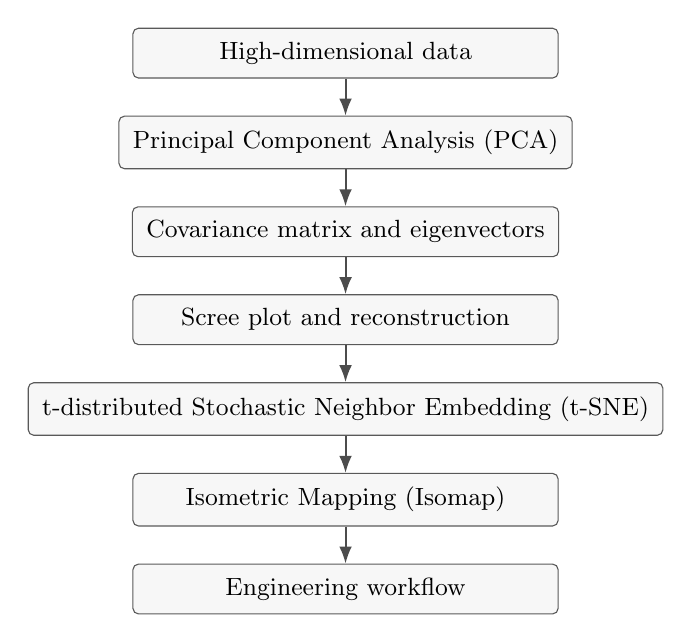
\begin{tikzpicture}[node distance=0.47cm]
\node[flowbox,minimum width=5.4cm] (a) {High-dimensional data};
\node[flowbox,minimum width=5.4cm,below=of a] (b) {Principal Component Analysis (PCA)};
\node[flowbox,minimum width=5.4cm,below=of b] (c) {Covariance matrix and eigenvectors};
\node[flowbox,minimum width=5.4cm,below=of c] (d) {Scree plot and reconstruction};
\node[flowbox,minimum width=5.4cm,below=of d] (e) {t-distributed Stochastic Neighbor Embedding (t-SNE)};
\node[flowbox,minimum width=5.4cm,below=of e] (f) {Isometric Mapping (Isomap)};
\node[flowbox,minimum width=5.4cm,below=of f] (g) {Engineering workflow};
\foreach \u/\v in {a/b,b/c,c/d,d/e,e/f,f/g}{\draw[flowarrow] (\u) -- (\v);}
\end{tikzpicture}%
}}

\title{Chapter~9~Dimensionality Reduction}
\author{Austin R.J. Downey}
\date{}

\begin{document}

\section{Machine Learning for Engineering Problem Solving}
\frame{\titlepage}

\section{Chapter~9~Dimensionality Reduction}

%------------------------------------------------
\begin{frame}{Chapter 9 Road Map}
\small
\begin{columns}[T,onlytextwidth]
\column{0.42\textwidth}

Dimensionality reduction replaces many measured variables with a few useful coordinates.

\vspace{0.35em}

\begin{itemize}
\item Why reduce dimension?
\item Principal Component Analysis (PCA)
\item Covariance matrix structure
\item Scree plots and reconstruction
\item t-distributed Stochastic Neighbor Embedding (t-SNE)
\item Isometric Mapping (Isomap)
\item Practical engineering use
\end{itemize}

\column{0.58\textwidth}
\centering
\DimRedRoadmap

\vspace{0.2em}
Road map from raw variables to reduced coordinates.
\end{columns}
\end{frame}

%------------------------------------------------
\begin{frame}{Why Reduce Dimension?}
\small
\begin{columns}[T,onlytextwidth]
\column{0.42\textwidth}

Many engineering variables are correlated.

\begin{itemize}
\item visualization in two or three dimensions
\item compression into fewer numbers
\item denoising by keeping repeatable structure
\item preprocessing before another model
\item exploration of clusters and outliers
\end{itemize}

\column{0.56\textwidth}
\centering

\includegraphics[width=\linewidth]{../figures/DimRed_overview.png}

\vspace{0.1em}
Many measured variables become a few useful coordinates.
\end{columns}
\end{frame}


%------------------------------------------------
\begin{frame}{Wine Data Matrix}
\small
\begin{columns}[T,onlytextwidth]
\column{0.38\textwidth}

A data matrix stores one sample per row.

\begin{itemize}
\item Wine has 178 samples
\item Wine has 13 measured features
\item rows: wine samples
\item columns: measured features
\item colors: standardized values
\item classes are grouped for display
\end{itemize}

\column{0.60\textwidth}
\centering

\includegraphics[width=\linewidth]{../figures/DimRed_wine_feature_matrix.png}

\vspace{0.1em}
The reduced representation should summarize this table with fewer coordinates.
\end{columns}
\end{frame}

%------------------------------------------------
\begin{frame}{Notation}
\small
\centering
\begin{tabular}{p{0.22\textwidth}p{0.64\textwidth}}
\toprule
\textbf{Symbol} & \textbf{Meaning} \\
\midrule
$\vct{x}^{(i)}\in\mathbb{R}^{d}$ & feature vector for sample $i$ \\
$\mat{X}\in\mathbb{R}^{m\times d}$ & data matrix; one row per sample \\
$m$ & number of samples \\
$d$ & number of original features \\
$r$ & number of reduced dimensions, with $r<d$ \\
$\mat{Z}\in\mathbb{R}^{m\times r}$ & reduced-coordinate matrix \\
$\mat{S}$ & covariance matrix \\
$\vct{u}_j$ & principal-component direction \\
$\lambda_j$ & variance explained by component $j$ \\
\bottomrule
\end{tabular}

\vspace{0.5em}
Vectors use arrows. Matrices use bold symbols.
\end{frame}

%------------------------------------------------
\begin{frame}{High-Dimensional Data Are Hard to Inspect}
\small
\begin{itemize}
\item Humans cannot directly inspect 13, 80, or 1000 dimensions.
\item Distances can become less informative as dimension grows.
\item Redundant features can make later models unstable.
\item Low-dimensional coordinates can reveal structure before modeling.
\item A two-dimensional plot is a summary, not the full data set.
\end{itemize}

\vspace{0.5em}
\begin{block}{Main idea}
Find a smaller coordinate system that preserves the structure needed for the task.
\end{block}
\end{frame}

\section{9.1 Principal Component Analysis}

%------------------------------------------------
\begin{frame}{Principal Component Analysis (PCA): Big Picture}
\small
\begin{columns}[T,onlytextwidth]
\column{0.43\textwidth}

Principal Component Analysis (PCA) finds linear directions of largest variance.

\begin{itemize}
\item first component: largest variance direction
\item second component: next largest orthogonal direction
\item components form a rotated coordinate system
\item keep only the first $r$ components to reduce dimension
\end{itemize}

\column{0.55\textwidth}
\centering

\includegraphics[width=\linewidth]{../figures/DimRed_pca_projection_geometry.png}

\vspace{0.1em}
PCA rotates the coordinate system toward the data spread.
\end{columns}
\end{frame}

%------------------------------------------------
\begin{frame}{Principal Component Analysis (PCA): Biggest Shadow}
\small
\begin{columns}[T,onlytextwidth]
\column{0.38\textwidth}

A useful intuition is the shadow analogy.

\begin{itemize}
\item project the data onto a line
\item measure the spread of the projection
\item rotate the line
\item choose the direction with the largest spread
\item that direction is the first principal component
\end{itemize}

\column{0.60\textwidth}
\centering

\includegraphics[width=0.9\linewidth]{../figures/DimRed_pca_shadow_projection.png}

\vspace{0.1em}
PCA finds the direction that casts the largest variance shadow.
\end{columns}
\end{frame}

%------------------------------------------------
\begin{frame}{Principal Component Analysis (PCA): Data Setup}
\small
For one sample,
\begin{equation*}
    \vct{x}^{(i)}
    =
    \begin{bmatrix}
    x^{(i)}_1\\
    x^{(i)}_2\\
    \vdots\\
    x^{(i)}_d
    \end{bmatrix}
    \in \mathbb{R}^{d}.
\end{equation*}

For a data set,
\begin{equation*}
    \mat{X}
    =
    \begin{bmatrix}
    - (\vct{x}^{(1)})^{\top} -\\
    - (\vct{x}^{(2)})^{\top} -\\
    \vdots\\
    - (\vct{x}^{(m)})^{\top} -
    \end{bmatrix}
    \in \mathbb{R}^{m\times d}.
\end{equation*}
\end{frame}

%------------------------------------------------
\begin{frame}{Principal Component Analysis (PCA): Center the Data}
\small
PCA studies variation around the mean.

\vspace{0.5em}
\begin{equation*}
    \bar{\vct{x}}
    =
    \frac{1}{m}\sum_{i=1}^{m}\vct{x}^{(i)}
\end{equation*}

\vspace{0.4em}
\begin{equation*}
    \mat{X}_{c}
    =
    \mat{X}-\vct{1}_{m}\bar{\vct{x}}^{\top}
\end{equation*}

\vspace{0.6em}
\begin{itemize}
\item $\bar{\vct{x}}$ is the mean feature vector.
\item $\vct{1}_{m}$ broadcasts the mean across all rows.
\item $\mat{X}_c$ is the centered data matrix.
\end{itemize}
\end{frame}

%------------------------------------------------
\begin{frame}{Principal Component Analysis (PCA): Covariance Matrix}
\small
The sample covariance matrix is
\begin{equation*}
    \mat{S}
    =
    \frac{1}{m-1}\mat{X}_{c}^{\top}\mat{X}_{c}.
\end{equation*}

\begin{itemize}
\item $\mat{S}\in\mathbb{R}^{d\times d}$
\item diagonal entries are feature variances
\item off-diagonal entries are feature covariances
\item correlated variables create off-diagonal structure
\item PCA finds special directions of this covariance matrix
\end{itemize}
\end{frame}

%------------------------------------------------
\begin{frame}{Principal Component Analysis (PCA): Covariance Matrix Structure}
\small
\begin{columns}[T,onlytextwidth]
\column{0.40\textwidth}

The covariance matrix is organized by features, not samples.

\begin{itemize}
\item $S_{jj}$ is the variance of feature $j$
\item $S_{ij}$ is the covariance of features $i$ and $j$
\item $S_{ij}=S_{ji}$
\item $\mat{S}$ is symmetric about the diagonal
\end{itemize}

\column{0.58\textwidth}
\centering

\includegraphics[width=\linewidth]{../figures/DimRed_covariance_matrix_structure.png}

\vspace{0.1em}
Diagonal entries are variances; off-diagonal entries are covariances.
\end{columns}
\end{frame}

%------------------------------------------------
\begin{frame}{Principal Component Analysis (PCA): Covariance Entries}
\small
Each entry of $\mat{S}$ is computed across samples.

\begin{equation*}
    S_{ij}
    =
    \frac{1}{m-1}
    \sum_{k=1}^{m}
    \left(X_{ki}-\bar{x}_{i}\right)
    \left(X_{kj}-\bar{x}_{j}\right)
\end{equation*}

\vspace{0.5em}
\begin{itemize}
\item $i$ and $j$ index features.
\item $k$ indexes samples.
\item $S_{ii}$ is the variance of feature $i$.
\item $S_{ij}=S_{ji}$, so the matrix is symmetric.
\end{itemize}
\end{frame}

%------------------------------------------------
\begin{frame}{Principal Component Analysis (PCA): Wine Covariance Matrix}
\small
\begin{columns}[T,onlytextwidth]
\column{0.39\textwidth}

For standardized data, the covariance matrix is equivalent to a correlation matrix.

\begin{itemize}
\item diagonal entries are one
\item red entries move together
\item blue entries move oppositely
\item PCA uses this structure to find components
\end{itemize}

\column{0.59\textwidth}
\centering

\includegraphics[width=0.88\linewidth]{../figures/DimRed_wine_covariance_heatmap.png}

\vspace{0.1em}
Covariance matrix for standardized Wine features.
\end{columns}
\end{frame}

%------------------------------------------------
\begin{frame}{Principal Component Analysis (PCA): Eigenproblem}
\small
PCA solves an eigenvalue problem on the covariance matrix.

\begin{equation*}
    \mat{S}\vct{u}_j=\lambda_j\vct{u}_j
\end{equation*}

\vspace{0.5em}
\begin{itemize}
\item $\vct{u}_j$ is the eigenvector and a principal-component direction.
\item $\lambda_j$ is the eigenvalue and the variance along that direction.
\item Eigenvalues are sorted from largest to smallest.
\end{itemize}

\vspace{0.5em}
\begin{equation*}
    \lambda_1\geq\lambda_2\geq\cdots\geq\lambda_d\geq 0
\end{equation*}
\end{frame}

%------------------------------------------------
\begin{frame}{Principal Component Analysis (PCA): What Gets Kept?}
\small
\begin{block}{Important distinction}
The eigenvectors define the new axes. The eigenvalues tell how much variance those axes explain.
\end{block}

\vspace{0.4em}
If we keep the first $r$ directions,
\begin{equation*}
    \mat{U}_{r}
    =
    \begin{bmatrix}
    \vct{u}_1 & \vct{u}_2 & \cdots & \vct{u}_r
    \end{bmatrix}
    \in \mathbb{R}^{d\times r}.
\end{equation*}

The reduced coordinates are
\begin{equation*}
    \mat{Z}=\mat{X}_{c}\mat{U}_{r}\in\mathbb{R}^{m\times r}.
\end{equation*}
\end{frame}

%------------------------------------------------
\begin{frame}{Principal Component Analysis (PCA): Standardization}
\small
PCA is sensitive to feature scale.

\vspace{0.5em}
\begin{equation*}
    X_{\mathrm{std},ij}
    =
    \frac{X_{ij}-\mu_j}{s_j}
\end{equation*}

\vspace{0.5em}
\begin{itemize}
\item use centered data when absolute units matter
\item use standardized data when features have different units
\item record the choice because it changes the components
\item many engineering data sets need standardization first
\end{itemize}
\end{frame}

%------------------------------------------------
\begin{frame}{Principal Component Analysis (PCA): Scree Plot}
\small
\begin{columns}[T,onlytextwidth]
\column{0.39\textwidth}

A scree plot shows how much variance each component explains.

\begin{itemize}
\item bars: individual explained variance
\item line: cumulative explained variance
\item large drop suggests low-dimensional structure
\item use validation and engineering judgment
\end{itemize}

\column{0.59\textwidth}
\centering

\includegraphics[width=\linewidth]{../figures/DimRed_wine_scree_plot.png}

\vspace{0.1em}
Scree plot for the standardized Wine data.
\end{columns}
\end{frame}

%------------------------------------------------
\begin{frame}{Principal Component Analysis (PCA): Explained Variance}
\small
The explained variance ratio for component $j$ is
\begin{equation*}
    \rho_j
    =
    \frac{\lambda_j}{\sum_{k=1}^{d}\lambda_k}.
\end{equation*}

\vspace{0.4em}
The cumulative explained variance after $r$ components is
\begin{equation*}
    R_r
    =
    \sum_{j=1}^{r}\rho_j.
\end{equation*}

\vspace{0.4em}
\begin{itemize}
\item common rules use 90\% or 95\% variance
\item low-variance components can still contain important fault information
\end{itemize}
\end{frame}

%------------------------------------------------
\begin{frame}{Principal Component Analysis (PCA): Scores for Wine Data}
\small
\begin{columns}[T,onlytextwidth]
\column{0.38\textwidth}

The first two PCA scores give a two-dimensional view.

\begin{itemize}
\item classes are not used to fit PCA
\item labels are shown for interpretation
\item overlap in two dimensions does not prove inseparability
\item useful first look before nonlinear methods
\end{itemize}

\column{0.60\textwidth}
\centering

\includegraphics[width=0.92\linewidth]{../figures/DimRed_wine_pca_scores.png}

\vspace{0.1em}
PCA score plot for the Wine data.
\end{columns}
\end{frame}

%------------------------------------------------
\begin{frame}{Principal Component Analysis (PCA): Loadings}
\small
\begin{columns}[T,onlytextwidth]
\column{0.39\textwidth}

Loadings show how original features contribute to components.

\begin{itemize}
\item each column of $\mat{U}_r$ is a loading vector
\item large magnitude means strong contribution
\item sign indicates direction on that component
\item loadings help interpret PCA scores
\end{itemize}

\column{0.59\textwidth}
\centering

\includegraphics[width=\linewidth]{../figures/DimRed_wine_pca_loadings.png}

\vspace{0.1em}
First two PCA loading vectors for the Wine data.
\end{columns}
\end{frame}

%------------------------------------------------
\begin{frame}{Principal Component Analysis (PCA): Reconstruction}
\small
The approximate reconstruction from $r$ components is
\begin{equation*}
    \hat{\mat{X}}
    =
    \mat{Z}\mat{U}_{r}^{\top}
    +
    \vct{1}_{m}\bar{\vct{x}}^{\top}.
\end{equation*}

\vspace{0.5em}
The reconstruction error is
\begin{equation*}
    \mat{E}=\mat{X}-\hat{\mat{X}}.
\end{equation*}

\vspace{0.5em}
\begin{itemize}
\item $r=d$ gives exact reconstruction for centered data
\item $r<d$ gives compression and information loss
\item reconstruction residuals can reveal unusual samples
\end{itemize}
\end{frame}

%------------------------------------------------
\begin{frame}{Principal Component Analysis (PCA): Reconstruction Error}
\small
\begin{columns}[T,onlytextwidth]
\column{0.40\textwidth}

More components reduce reconstruction error.

\begin{itemize}
\item one component gives strong compression
\item more components keep more detail
\item the curve helps choose $r$
\item reconstruction residuals are useful for monitoring
\end{itemize}

\column{0.58\textwidth}
\centering

\includegraphics[width=\linewidth]{../figures/DimRed_pca_reconstruction_error.png}

\vspace{0.1em}
Reconstruction error decreases as more components are kept.
\end{columns}
\end{frame}

%------------------------------------------------
\begin{frame}{Principal Component Analysis (PCA): Denoising}
\small
\begin{columns}[T,onlytextwidth]
\column{0.38\textwidth}

PCA can denoise when repeatable structure is low-dimensional.

\begin{itemize}
\item fit PCA to many related signals
\item keep dominant components
\item reconstruct from the retained scores
\item discarded directions often contain noise
\end{itemize}

\column{0.60\textwidth}
\centering

\includegraphics[width=\linewidth]{../figures/DimRed_pca_reconstruction_denoising.png}

\vspace{0.1em}
Noisy measurements can be reconstructed from a small PCA subspace.
\end{columns}
\end{frame}

%------------------------------------------------
\begin{frame}{Principal Component Analysis (PCA): Preprocessing}
\small
\begin{columns}[T,onlytextwidth]
\column{0.38\textwidth}

PCA can feed a later supervised model.

\begin{itemize}
\item standardize features
\item project onto $r$ components
\item train the downstream model
\item choose $r$ using validation behavior
\item fit preprocessing only on training data
\end{itemize}

\column{0.60\textwidth}
\centering

\includegraphics[width=\linewidth]{../figures/DimRed_pca_preprocessing_accuracy.png}

\vspace{0.1em}
Wine classification after PCA preprocessing.
\end{columns}
\end{frame}

%------------------------------------------------
\begin{frame}{Principal Component Analysis (PCA): Residuals for Monitoring}
\small
For sample $i$, a squared reconstruction residual is
\begin{equation*}
    Q_i
    =
    \left\|\vct{x}^{(i)}-\hat{\vct{x}}^{(i)}\right\|_2^2.
\end{equation*}

\vspace{0.5em}
\begin{itemize}
\item small residual: sample fits the retained PCA subspace
\item large residual: sample is not well reconstructed
\item possible causes include faults, sensor problems, or new operating conditions
\item the residual is a screening statistic, not proof of a specific failure
\end{itemize}
\end{frame}

\section{9.2 Nonlinear Visualization Methods}

%------------------------------------------------
\begin{frame}{t-distributed Stochastic Neighbor Embedding (t-SNE): Idea}
\small
\begin{columns}[T,onlytextwidth]
\column{0.42\textwidth}

t-distributed Stochastic Neighbor Embedding (t-SNE) is a nonlinear visualization method.

\begin{itemize}
\item preserves local neighborhoods
\item usually produces 2D or 3D plots
\item useful for exploratory visualization
\item not designed to preserve global distances
\item random seed and parameters matter
\end{itemize}

\column{0.56\textwidth}
\centering

\includegraphics[width=\linewidth]{../figures/DimRed_tsne_local_neighbors.png}

\vspace{0.1em}
t-SNE emphasizes local neighborhoods.
\end{columns}
\end{frame}

%------------------------------------------------
\begin{frame}{t-distributed Stochastic Neighbor Embedding (t-SNE): Neighbor Probabilities}
\small
In the original space, nearby points get larger neighbor probabilities.

\scriptsize
\begin{equation*}
    p_{j|i}
    =
    \frac{
    \exp\left(-\left\|\vct{x}^{(i)}-\vct{x}^{(j)}\right\|_2^2/(2\sigma_i^2)\right)
    }
    {
    \sum_{k\neq i}\exp\left(-\left\|\vct{x}^{(i)}-\vct{x}^{(k)}\right\|_2^2/(2\sigma_i^2)\right)
    }.
\end{equation*}
\normalsize

\vspace{0.4em}
In the low-dimensional map, t-SNE defines another set of neighbor probabilities and moves points to make the two probability patterns similar.

\begin{itemize}
\item close high-dimensional neighbors should remain close
\item far-away global distances are less reliable
\end{itemize}
\end{frame}

%------------------------------------------------
\begin{frame}{t-distributed Stochastic Neighbor Embedding (t-SNE): Perplexity}
\small
\begin{columns}[T,onlytextwidth]
\column{0.39\textwidth}

Perplexity controls the effective neighborhood size.

\begin{itemize}
\item small perplexity emphasizes local detail
\item large perplexity uses broader neighborhoods
\item layouts can change with perplexity
\item compare several settings before making claims
\end{itemize}

\column{0.59\textwidth}
\centering

\includegraphics[width=\linewidth]{../figures/DimRed_tsne_wine_perplexity.png}

\vspace{0.1em}
The same Wine data can produce different t-SNE layouts.
\end{columns}
\end{frame}

%------------------------------------------------
\begin{frame}{t-distributed Stochastic Neighbor Embedding (t-SNE): Cautions}
\small
\begin{itemize}
\item t-SNE is best treated as an exploratory plotting tool.
\item Cluster sizes in the plot are not calibrated physical sizes.
\item Distance between clusters is not a reliable physical distance.
\item Different random seeds can give different layouts.
\item Fit PCA first when the original feature count is very large.
\end{itemize}

\vspace{0.5em}
\begin{block}{Teaching phrase}
t-SNE is good for asking ``who is near whom?'' It is not good for measuring exact distances between groups.
\end{block}
\end{frame}

%------------------------------------------------
\begin{frame}{Isometric Mapping (Isomap): Graph-Based Idea}
\small
\begin{columns}[T,onlytextwidth]
\column{0.39\textwidth}

Isometric Mapping (Isomap) is a graph-based manifold method.

\begin{itemize}
\item connect nearby samples
\item compute shortest paths on the graph
\item preserve graph distances in a low-dimensional map
\item useful for curved low-dimensional structure
\item included in \texttt{scikit-learn}
\end{itemize}

\column{0.59\textwidth}
\centering

\includegraphics[width=\linewidth]{../figures/DimRed_isomap_swiss_roll.png}

\vspace{0.1em}
Isomap can unroll some curved synthetic manifolds.
\end{columns}
\end{frame}

%------------------------------------------------
\begin{frame}{Comparing PCA, t-SNE, and Isomap}
\small
\begin{columns}[T,onlytextwidth]
\column{0.37\textwidth}

The methods preserve different structure.

\begin{itemize}
\item PCA: global linear variance
\item t-SNE: local neighborhoods
\item Isomap: graph-based distances
\item none of these plots proves a classifier works
\item validate on the engineering task
\end{itemize}

\column{0.61\textwidth}
\centering

\includegraphics[width=\linewidth]{../figures/DimRed_method_comparison_wine.png}

\vspace{0.1em}
The same Wine data shown with three dimensionality-reduction assumptions.
\end{columns}
\end{frame}

%------------------------------------------------
\begin{frame}{Practical Workflow}
\small
\begin{columns}[T,onlytextwidth]
\column{0.40\textwidth}

A safe workflow avoids leakage.

\begin{itemize}
\item define the purpose
\item split the data
\item fit scaling on training data
\item fit PCA or reducer on training data
\item inspect plots and residuals
\item validate the downstream task
\end{itemize}

\column{0.58\textwidth}
\centering

\includegraphics[width=\linewidth]{../figures/DimRed_workflow.png}

\vspace{0.1em}
Fit preprocessing with training data only.
\end{columns}
\end{frame}

%------------------------------------------------
\begin{frame}{scikit-learn Implementation Pattern}
\small
For a supervised workflow, use a pipeline.

\vspace{0.5em}
\begin{equation*}
\texttt{StandardScaler()}
\quad\rightarrow\quad
\texttt{PCA(n\_components=r)}
\quad\rightarrow\quad
\texttt{LogisticRegression()}
\end{equation*}

\vspace{0.5em}
\begin{itemize}
\item \texttt{fit}: estimate parameters from training data
\item \texttt{transform}: apply an already fitted transformation
\item \texttt{fit\_transform}: fit and transform the same data
\item choose $r$ using validation behavior
\item reuse the fitted scaler and PCA directions for future samples
\end{itemize}
\end{frame}

%------------------------------------------------
\begin{frame}{Common Mistakes}
\small
\begin{itemize}
\item fitting scaling or PCA before the train-test split
\item treating t-SNE cluster distances as physical distances
\item choosing PCA components only from a fixed variance rule
\item ignoring units and feature scaling
\item using a nice two-dimensional plot as proof of model performance
\item forgetting that rare but important events can be low-variance
\end{itemize}
\end{frame}

%------------------------------------------------
\begin{frame}{Summary}
\small
Dimensionality reduction summarizes high-dimensional data with fewer coordinates.

\begin{itemize}
\item Principal Component Analysis (PCA) uses the covariance matrix.
\item PCA eigenvectors define principal-component directions.
\item PCA eigenvalues tell how much variance each direction explains.
\item Scree plots help choose the number of components.
\item Reconstruction supports compression, denoising, and residual monitoring.
\item t-distributed Stochastic Neighbor Embedding (t-SNE) shows local neighborhoods.
\item Isometric Mapping (Isomap) gives a graph-based manifold view.
\end{itemize}

\vspace{0.4em}
Use reduced coordinates only after checking what structure the method preserves.
\end{frame}

\end{document}
